\section{Probabilistic inference for control}
\label{s:pilco}
The controller is a function $\pi(x_{t})=u_{t}$, which takes a current state $x_{t}$ of the system and outputs a new action $u_{t}$ to be applied to the system. The system will then evolve according to its dynamics function $f$:
\begin{equation}
x_{t+1}=f(x_{t}, u_{t})
\end{equation}
Given the previous state $x_{t}$ and the applied action $u_{t}$, the dynamics function $f$ returns the new state of the system. Furthermore, each single state of the system $x_{t}$ has an associated cost $c(x_{t})$\ (e.g., the distance between the tip of pendulum and the upright position). For the given controller $\pi$, the total cost associated with the evolution of the system from the uncertain state i.e. $x_{1} \sim \mathcal{N}(\mu, \sigma^2)$ can be defined as $J^{\pi}$:
\begin{equation}
J^{\pi}=\sum_{t=1}^{T} \mathbb{E}[c(x_{t})]
\end{equation}
PILCO \cite{deisenroth2011pilco} is a probabilistic inference framework for learning the $\pi$ controller function which minimizes its $J^{\pi}$ total cost. 

\noindent The dynamics function of the system $f(x_{t}, u_{t})$ can be redefined as $f(\overline{x}_{t})$, where $\overline{x}_{t} \equiv [x_{t}, u_{t}]$. This nonlinear dynamics $f(\overline{x}_{t})$ can be modeled by Gaussian Processes. Different dynamics models involving Gaussian Processes are detailed in the next section \ref{s:pilco:dyn}. Given the dynamics model and the controller $\pi$, the $J^{\pi}$ total cost of the policy can be approximated by propagating uncertainty \cite{candela2003propagation} through controller and dynamics functions. 

\noindent To calculate the distribution over the next state  from the distribution over the current state: $p((x_{t}) -> p(x_{t+1})$: First, the uncertain state $x_{t} \sim \mathcal{N}(\mu, \sigma^2)$ can be propagated through the $\pi$ controller function to get a distribution over the next action: $p(u_{t})$. If the controller function is nonlinear, the output distribution is approximated as Gaussian distribution by moment matching. Next, by computing the covariance between $x_{t}$ and $u_{t}$, we construct the joint normal distribution over $x_{t}$ and $u_{t}$ defined as $p(\overline{x}_{t})$. This distribution is then propagated through the dynamics function $x_{t+1}=f(\overline{x}_{t})$. Again, since $f$ function is nonlinear, the output distribution is not Gaussian and needs to be approximated by moment matching. 

\noindent The one-step uncertainty propagation may be extended to calculate the distribution over all the states: $p(x_{1}, x_{2}, x_{3}...x_{T})$. Having the distribution over all the states, the total cost $J^{\pi}$ of the current controller can be directly computed. To learn successful controller, PILCO conditions the $\pi$ controller on its parameters $\theta$: $\pi(x_{t}|\theta)=u_{t}$. Then, the derivatives of the total cost with respect to the controller parameters $\frac{\partial J^{\pi}}{\partial \theta}$ are computed and used for optimization of $\theta$ parameters of the controller. The details of this approach can be found in Deisenroth and Rasmussen \cite{deisenroth2011pilco}.

\subsection{Dynamics model}
\label{s:pilco:dyn}

The dynamics model maps the current state $x_{t}$ and the applied action $u_{t}$ to the next state $x_{t+1}$:  $x_{t+1}=f(\overline{x}_{t})$,  where $\overline{x}_{t} \equiv [x_{t}, u_{t}]$. It is worth noticing that for the dynamics model, the applied action $u_{t}$ is treated as any other state variable. Gaussian Processes\ (GP) are chosen for modeling the dynamics, since the dynamics of inverted pendulum is nonlinear.

\noindent The single evolution of the system generates the following samples for the dynamics model: $[\overline{x}_{1}, x_{2}], [\overline{x}_{2}, x_{3}], [\overline{x}_{3}, x_{4}] [\overline{x}_{4}, x_{5}]...[\overline{x}_{T-1}, x_{T}]$, where the first position is the input to the dynamics model and the second is its output. There is a noise on inputs as well as outputs. The standard GP regression model presented in the section \ref{s:pilco:gpr} assumes the noisy outputs, but not the noisy inputs. The noise on the inputs may be ignored, so the samples can be fitted directly to the GP regression model as if the inputs were not noisy. Another approach is to filter first the noisy inputs passed to the dynamics model. The input of the sample at time $t$ is also the output of the sample at time $t-1$. The predictive distribution of the GP for the input at time $t-1$ can be used to filter the input at time $t$. This will result in the distribution on the input, which may be propagated through GP. The output distribution at time $t$ is approximated to normal distribution by moment matching. This idea is embodied in the Direct Method for Gaussian Processes Time-Series model described in the section \ref{s:pilco:ssm}.

\subsubsection{Gaussian Processes for Regression}
\label{s:pilco:gpr}
The Gaussian Processes\ (GP) model the distribution over the functions. The predictive distribution $y_*$ at any test input $x_{*}$ is Gaussian and depends on all of the training points $({\bf x}, {\bf y})$:
\begin{equation} \label{eq:gpr:preddistr}
\begin{split}
p(y_*|x_*,{\bf x},{\bf y}, \mathcal{M}_i) \sim {\cal N}\big(&{\bf k}(x_*,{\bf x})^\top [K+\sigma_{\rm noise}^2I]^{-1}{ \bf y}, \\
& k(x_*,x_*)+\sigma_{\rm noise}^2-{\bf k}(x_*,{\bf x})^\top [K+\sigma_{\rm noise}^2I]^{-1}{\bf k}(x_*,{\bf x})
\end{split}
\end{equation}
where $k(x,x')$ is a covariance function and $K$ is a covariance matrix in which $K_{ij}$ element equals to $k({\bf x}_{i}, {\bf x}_{j})$. The example of $k(x,x')$ is a squared exponential covariance function:
\begin{equation} \label{eq:gpr:covse}
k_{SE}(x,x') = v^2\exp\big(-\displaystyle\frac{(x-x')^2}{2\ell^2}\big)
\end{equation}
where the hyperparamaters are $v$-signal and $\ell$-lenghtscale\ (also, $\sigma_{\rm noise}$ in the equation \ref{eq:gpr:preddistr} is another hyperparameter).  The lengthscale $\ell$ describes how much two $x$ points should covary depending on the distance between them. If the lengthscale $\ell$ is small, the two $x$ points covary only if they are close to each other. The squared exponential is a stationary covariance function, which means that how two points covary depends only on the difference between them\ (i.e. $x-x'$), not on their absolute values. In this dissertation, the $x$ inputs are multidimensional\ (as the state of the inverted pendulum has more than one variable). We use automatic relevance determination\ (ARD) covariance function, which is a multidimensional equivalent of squared exponential covariance function while having separate $\ell$ lengthscale hyperparamaters for each dimension. 

\noindent The predictive distribution for the test input $x_{*}$ given in the equation \ref{eq:gpr:preddistr} is conditioned on $\mathcal{M}_i$, which is a linear contribution of the GP model in this dissertation. The predictive distribution for the test input $x_{*}$, which includes the linear contribution will have, additionally, its mean shifted by a linear component: $w^\top x_{*}+b$.  It is worth highlighting the fact that the GP model is a nonparametric model. The distribution over the functions is expressed directly by all of the training points.  In a sense, a single training point is a "parameter" of the model. The more training points there are available, the larger the amount of "parameters" of the GP model is.

\noindent The Figures \ref{fig:gpr:gp0}-\ref{fig:gpr:gp3} shows how the predictive distribution for all $x_{*}$ test inputs change with more training points being available. The GP with a squared exponential covariance function and the hyperparameters: lengthscale $\ell=0.5$, signal $s=1$ and the noise  $\sigma_{\rm noise}^2=0.01$, is used. This GP model does not have a linear component. The Figure \ref{fig:gpr:gp0} shows the predictive distribution for $x_{*}$ if no training points are available. The predictive distribution is the same for any test input: the mean is equal to zero and the variance is equal to $1.01$, where $s^2+\sigma_{\rm noise}^2=1.01$\ (the grey area on the diagrams corresponds to the variance being multiplied by $2$). Any new training point changes the mean and the variance of the test points in its neighborhood, where the lengthscale parameter $\ell$ defines how big the affected neighborhood is. On the Figure \ref{fig:gpr:gp3}, we can see that the GP model remains uncertain about the regions of the function, in which there were no training points. The mean and the variance for $x=-3$ is the same if there are three training points\ (Figure \ref{fig:gpr:gp3}) or no training points\ (Figure \ref{fig:gpr:gp0}).

\begin{figure}[!ht]
    \centering
    \begin{floatrow}
    \ffigbox[\FBwidth][\FBheight][t]{\includegraphics[width=60mm,scale=0.6]{plots/gp_nosamples}}{\caption{GP distribution over the functions if no training points are available.}\label{fig:gpr:gp0}}
    \ffigbox[\FBwidth][\FBheight][t]{\includegraphics[width=60mm,scale=0.6]{plots/gp_1sample}}{\caption{GP distribution over the functions if one training point is available.}\label{fig:gpr:gp1}}
    \end{floatrow}
    \begin{floatrow}
    \ffigbox[\FBwidth][\FBheight][t]{\includegraphics[width=60mm,scale=0.6]{plots/gp_2samples}}{\caption{GP distribution over the functions if two training points are available.}\label{fig:gpr:gp2}}
    \ffigbox[\FBwidth][\FBheight][t]{\includegraphics[width=60mm,scale=0.6]{plots/gp_3samples}}{\caption{GP distribution over the functions if three training points are available.}\label{fig:gpr:gp3}}
    \end{floatrow}
\end{figure}

\noindent The calculation of predictive distribution for the input $x_{*}$\ (equation {eq:gpr:preddistr}) involves the inversion of $[K+\sigma_{\rm noise}^2I]$ matrix. The matrix has a size of $NxN$, where $N$ is the amount of training inputs. This means that the inversion of the matrix itself has a time complexity of $\Theta(N^3)$. However, $[K+\sigma_{\rm noise}^2I]^{-1}$ can be precomputed in the training phase, since it does not depend on the test input $x_{*}$. This will result in $\Theta(N^2)$ time complexity of the prediction\ (multiplication of a matrix with a vector in variance term). Moreover, the training of the GP model involves many $\Theta(N^3)$ operations. Hyperparameters are trained by gradient based optimization of the marginal likelihood, which involves the inversion of the $K$ matrix. For hyperparamters training, this operation can't be precomputed, since $K$ matrix itself depends on the hyperparameters. More details on the inference and training in Gaussian Processes can be found in Rasmussen \cite{rasmussen2006gaussian}.

\subsubsection{Sparse Gaussian Processes}
\label{s:pilco:sgpr}

The full GP model presented in the previous section \ref{s:pilco:gpr} can be approximated by replacing the $N$ training points with $M$ pseudo points, where $M<<N$. The Figure \ref{fig:sgpr:fullgp} shows the predictive distribution of the trained GP model expressed by 9 training points, whereas the predictive distribution on the Figure \ref{fig:sgpr:sparsegp} is expressed by only using 3 pseudo points. In this toy example, we can see that both GPs model very similar predictive distribution tough they use different amount of points to express it. Second GP model used pseudo points, which are synthetic data. Pseudo points\ (i.e. pseudo inputs $\underline{x}$ and pseudo targets $\underline{f}$) are optimized to approximate the full GP. Pseudo targets $\underline{f}$ are not noisy, since $\underline{f}$ targets are not real observations, whereas the outputs $y$ of the training points for the full GP model are noisy. 

\begin{figure}[!ht]
    \centering
    \begin{floatrow}
    \ffigbox[\FBwidth][\FBheight][t]{\includegraphics[width=60mm,scale=0.6]{plots/gp_full}}{\caption{The predictive distribution of the full GP model expressed by 9 training points.}\label{fig:sgpr:fullgp}}
    \ffigbox[\FBwidth][\FBheight][t]{\includegraphics[width=60mm,scale=0.6]{plots/gp_sparse}}{\caption{The similar predictive distribution of another GP model expressed by only 3 pseudo points.}\label{fig:sgpr:sparsegp}}
    \end{floatrow}
\end{figure}
 
\noindent The Fully Independent Training Conditional\ (FITC) approximation \cite{snelson2006sparse} learns the pseudo points in the following way. Assuming that the pseudo inputs $\underline{x}$ are known, it makes inference on the distribution over the pseudo targets $\underline{f}$. As the inference, we mean applying the Bayes rule to the prior on pseudo targets $\underline{f}$ and the likelihood of the training dataset $({\bf x}, {\bf y})$. Then, the posterior distribution over $\underline{f}$ can be integrated out to calculate the predictive distribution of the model for the test input $x_{*}$. To find the pseudo inputs $\underline{x}$, the gradient based optimization is applied to the marginal likelihood of the training dataset $({\bf x}, {\bf y})$. The details on the training of the FITC model can be found in Snelson and Ghahramani \cite{snelson2006sparse}. The model reduces the prediction time of the full GP from $\Theta(N^2)$ to $\Theta(M^2)$ and its training time from $\Theta(N^3)$ to $\Theta(M^2*N)$.

\noindent The FITC model can be also converted into a simpler parametric model. By taking the mean of the posterior distribution over $\underline{f}$ pseudo targets in FITC model and defining it as $\underline{\underline{f}}$, we get the parametric pseudo points: $(\underline{\underline{x}}, \underline{\underline{f}})$, where $\underline{\underline{x}} \equiv \underline{x}$. Those parametric pseudo points along with the learned hyperparameters in FITC can be directly used to model the new GP model. The prediction time of that model remains to have $\Theta(M^2)$ time complexity, but any retraining of this parametric GP model will take $\Theta(M^3)$\ (training of the Sparse GP model takes $\Theta(M^2*N)$). The Figure \ref{fig:sgpr:fullgp} shows the full GP model, whereas its parametric equivalent can be seen on the Figure \ref{fig:sgpr:sparsegp}. 

\subsubsection{Direct Method for Gaussian Processes Time-Series model}
\label{s:pilco:ssm}

To account for the noise in the inputs, the Direct Method for Gaussian Processes Time-Series model \cite{mch-thesis} can be used for modeling the dynamics. The model is shown on the Figure \ref{fig:dtsm:basic}. The latent state $x_{t}$, which is a normally distributed random variable, generates the observation $y_{t}$ while adding the Gaussian observation noise $\epsilon_{on}$ to it. Then, the latent state $x_{t}$ at time $t$ can be propagated through the parametric GP to achieve the latent state at time $t+1$, $x_{t+1}$. The Gaussian process noise, $\epsilon_{pn}$ is first added to the next latent state, $x_{t+1}$. The latent state at time $t+1$ can generate the observation $y_{t+1}$. The process may be continued till the last observation of the system $y_{T}$, which is the end of the rollout. 

\noindent The parametric GP model was presented in the previous section \ref{s:pilco:sgpr}. \underline{\underline{x}}\ and\ \underline{\underline{f}} are, respectively, the pseudo inputs and the pseudo targets of the parametric GP model. Since the parametric GP models the nonlinear function, the output distribution for propagating the Gaussian latent state $x_{t}$ as input is no longer Gaussian. That output distribution is approximated to normal distribution by moment matching. Consequently, each of the latent states $x_{t}$ is normally distributed.

\begin{figure}[H]
\centering
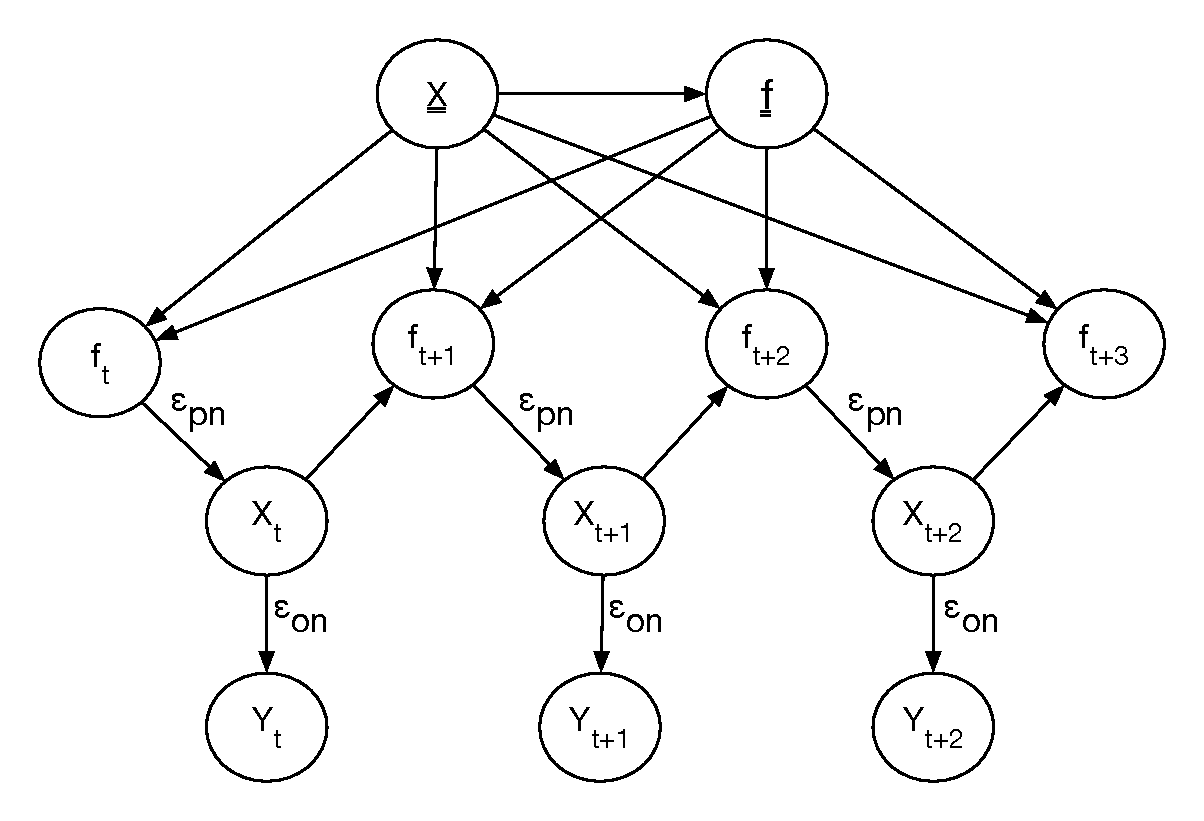
\includegraphics[width=1\textwidth, scale=1]{plots/ssm_model}
\caption{\label{fig:dtsm:basic}The Direct Method for Gaussian Processes Time-Series model in which: $y_{t}$ is a noisy observation of the state at time $t$; $x_{t}$ is a distribution over the latent state at time $t$; \underline{\underline{x}}\ and\ \underline{\underline{f}}\ are the pseudo inputs and the pseudo targets of the parametric GP model; $\epsilon_{pn}$ and $\epsilon_{on}$ stand for process and observation noise respectively.}
\end{figure}

\noindent There are the three levels of noise in the model: observation noise $\epsilon_{on}$, process noise $\epsilon_{pn}$ and the noise hyperparameter of the parametric GP $\sigma_{\rm noise}$. Only observation noise $\epsilon_{on}$ is not being propagated to the next latent state $x_{t+1}$. Process noise $\epsilon_{pn}$ and the noise of the parametric GP $\sigma_{\rm noise}$ are being added to all of the latent states $x_{1:T}$.

\noindent We can also write the marginal likelihood of the observations under the Direct Method for Gaussian Processes Time-Series. We define: $\theta := [\underline{\underline{x}}, \underline{\underline{f}}, \epsilon_{pn}, \epsilon_{on}, GP_{hyp}]$, where $GP_{hyp}$ stands for the hyperparameters of the parametric GP model. Then, the likelihood for the model can be written in the following way:
	
\begin{equation} \label{eq:ssm:lik}
\begin{split}
p(y_{1:T}|\theta) & = p(y_{1:T}|x_{1:T},\theta) p(x_{1:T}|\theta) \\
& =	p(y_{1:T}|x_{1:T},\theta) p(x_{1}| \theta) \prod_{t=2}^{T} p(x_{t}|x_{t-1}, \theta)
\end{split}
\end{equation}

\noindent The latent state at time $t$ depends only on the previous latent state at time $t-1$, not on any of the earlier latent states $x_{1:t-2}$. This Markovian property makes the Direct Method for Gaussian Processes Time-Series model tractable. The parameters $\theta$ are trained by gradient based optimization of the marginal likelihood \ref{eq:ssm:lik}. A single propagation of uncertain input through a parametric GP with precomputed inverse of covariance matrix has a time complexity of $\Theta(M^2)$, where $M$ is the amount of pseudo points. The derivative of the mean and variance of the output distribution with respect to the hyperparamaters and the pseudo targets of the parametric GP model can be also calculated in $\Theta(M^2)$ time. This uncertain input propagation needs to be conducted ${T}$ for each rollout (i.e. $[x_{1},x_{2}, x_{3},...x_{T}$). Therefore, the total time complexity of the single training iteration will be $\Theta(R*T*M^2)$, where $R$ is the amount of the rollouts. However, the operation can be made in parallel, since the computation of the prediction and derivatives for each of the rollouts are independent\ (the respective derivatives only need to be added at the end). More details on the Direct Method for Gaussian Processes Time-Series model can be found in McHutchon, Chapter 3 \cite{mch-thesis}.

\noindent In the above Direct Method for Gaussian Processes Time-Series model, only the hyperparameters and the pseudo targets are trained. The pseudo inputs may be pre-trained in the GP model which assumes noise-free inputs\ (e.g., full GP or sparse GP converted to the parametric GP). In this dissertation, the Direct Method for Gaussian Processes Time-Series model was extended to also optimize the pseudo inputs. The computation of the derivatives of the parametric GP's output distribution $x_{t+1}$ for an uncertain input $x_{t}$ with respect to the pseudo inputs has a time complexity of $\Theta(M^3)$. This makes the single iteration of the training procedure to have the time complexity of $\Theta(R*T*M^3)$. 

\begin{figure}[H]
\centering
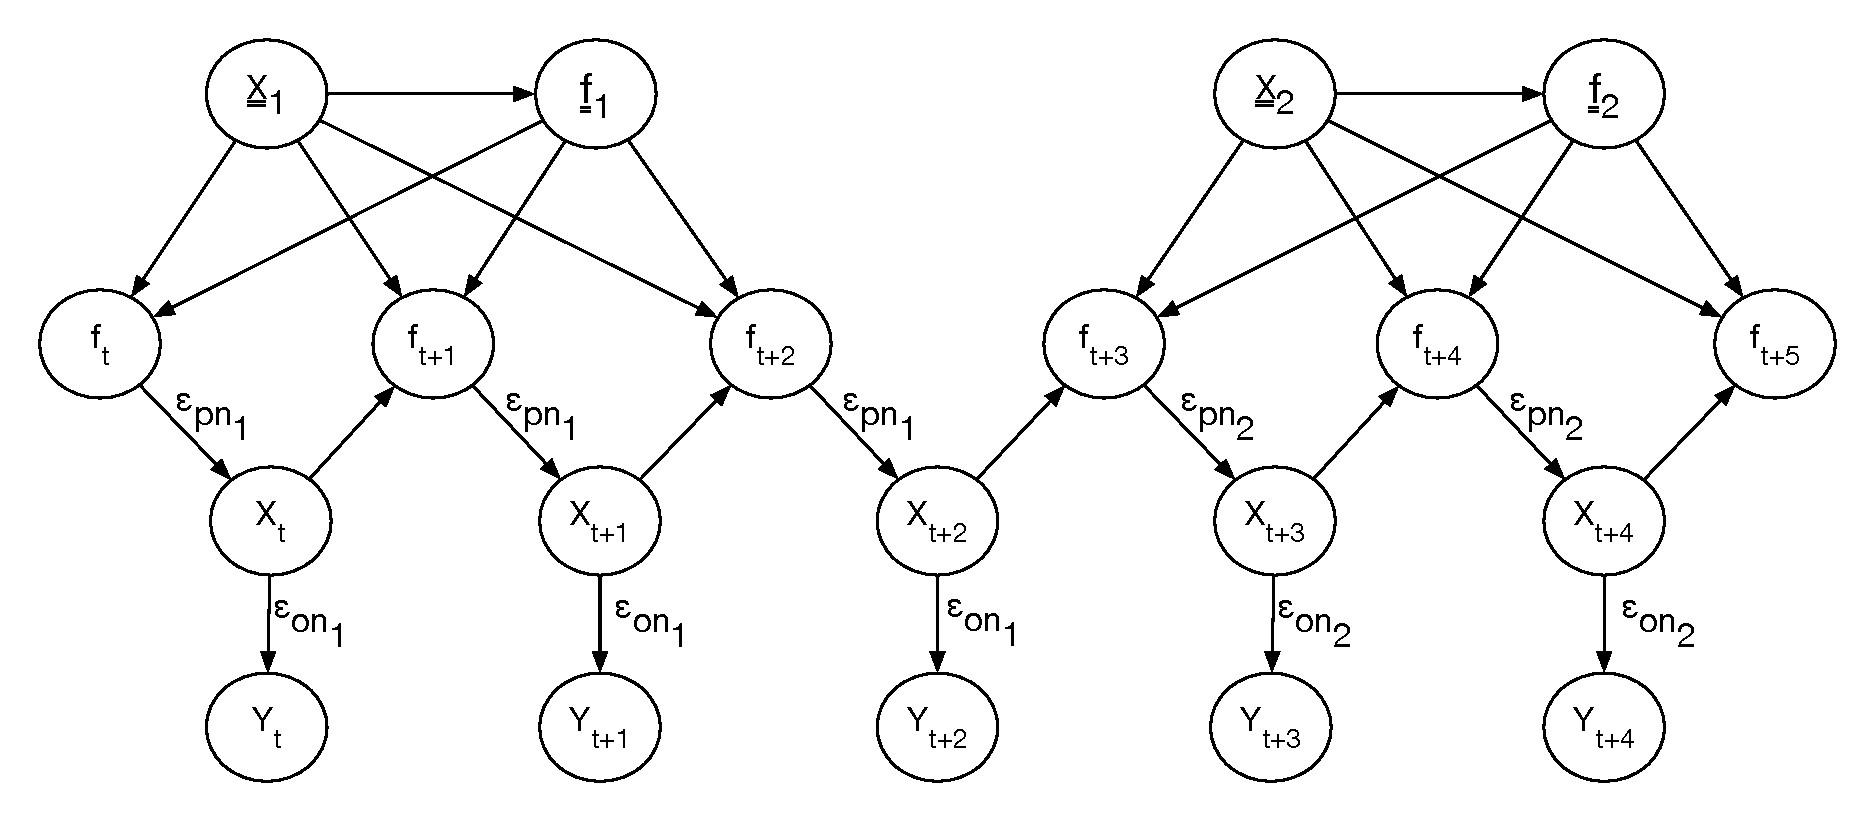
\includegraphics[width=1\textwidth, scale=1]{plots/ssm_models}
\caption{\label{fig:dtsm:twogps}The Direct Method for Gaussian Processes Time-Series model with two parametric GP models.}
\end{figure}

\noindent The Direct Method for Gaussian Processes Time-Series model may also use more than one parametric GP. The Figure \ref{fig:dtsm:twogps} shows the model in which two parametric GPs are used\ (there are two sets of pseudo points $\underline{\underline{x}}_1, \underline{\underline{f}}_1$ and $\underline{\underline{x}}_2, \underline{\underline{f}}_2$). In this model, there are also two separate sets of noise levels\ (process noises: $\epsilon_{pn_{1}}$ and $\epsilon_{pn_{2}}$, observation noises: $\epsilon_{on_{1}}$ and $\epsilon_{on_{2}}$). Although twice as many pseudo inputs are used, the output distribution for the uncertain input is calculated as many times as if the single parametric GP model was used. The time complexity of one training iteration remains to be $\Theta(R*T*M^3)$. However, there are twice as many parameters to optimize, which influences the amount of training iteration needed to find the sufficient approximation of the Hessian matrix in the BFGS algorithm used in this dissertation.

\noindent In the new model, the different dynamics models\ (i.e. parametric GPs) are used depending on which time step the rollout is at. This assumption seems unreal, since the physics of motion of the inverted pendulum does not change depending on time. However, time $t$ itself may be strongly correlated with the latent state $x_{t}$ e.g., at time $t_{k}$ the pendulum is usually having a high, positive angular velocity. By using different dynamics depending on time $t$, we effectively split the domain of the latent state $x_{t}$ into the few subdomains and use separate dynamics model for each of them. The switching between the different parametric GP models could also happen directly basing on the current latent state $x_{t}$. Those issues are further discussed, when the model is applied to the double inverted pendulum problem in the section \ref{s:exps:double:dyns}.

\noindent The Direct Method for Gaussian Processes Time-Series model requires to specify the amount of the pseudo points $(\underline{\underline{x}}, \underline{\underline{f}})$ being used. As mentioned earlier, the pseudo inputs\ \underline{\underline{x}}\ are pre-trained using the Sparse GP model. We compare the marginal likelihood of the observed data under the Sparse GP and the full GP models to determine how many pseudo points to use. If the marginal likelihood under the Sparse GP model is worse, more pseudo points should be added to the Gaussian Processes Time-Series model.

\subsection{Policy model}
\label{s:pilco:pol}
The closed-loop controller $\pi$ chooses the action $u$ to be applied depending on the current state of the system: $\pi(x_{t})=u_{t}$. As described earlier, to evaluate the policy, the uncertain state $p(x_{t})$ is propagated through the controller. This gives the distribution over the action $p(u_{t})$. The controller also keeps track on how the variables of the state $x_{t}$ covary with the action $u_{t}$. This way, the predictive variance on the future state of the system is being controlled. The Figure \ref{fig:pol:variancext} shows the linear relationship between the uncertain current state $x_{t}$ and the action $u_{t}$. The applied action results in the reduced variance on state $x_{t+1}$ on the Figure \ref{fig:pol:variancext1}. The variance is also being added to the system, since the controller performs a specific task like swinging up the pendulum.

\begin{figure}
    \centering
    \begin{floatrow}
    \ffigbox[\FBwidth][\FBheight][t]{\includegraphics[width=60mm,height=40mm]{plots/variance_state_t}}{\caption{The uncertain state $x_{t}$ with standard deviation equalled to $0.5$. There is a linear relationship between the state  $x_{t}$ and the applied action $u_{t}$ chosen by the closed-loop controller.}\label{fig:pol:variancext}}
    \ffigbox[\FBwidth][\FBheight][t]{\includegraphics[width=60mm,height=40mm]{plots/variance_state_t_1}}{\caption{The uncertain state $x_{t+1}$ with standard deviation equalled to $0.2$}\label{fig:pol:variancext1}}
    \end{floatrow}
\end{figure}

\noindent The range of actions which can be applied to the real system is limited. The inverted pendulum physical apparatus used in this dissertation allows to pass the force values between $-10$ and $10$. That's why the unlimited policy output $u$ is saturated through the squashing function $sat(u)$. This operation gives action $\overline{u}$ in the requested range:
\begin{equation}
\overline{u} = sat(u) = 10 * \frac{9 * sin(u) + sin (3 * u)}{8}
\end{equation}

\subsubsection{Radial Basis Function network}
\label{s:pilco:rbf}
The radial basis function\ (RBF) network models the nonlinear function as the sum of radial basis function units:
\begin{equation}
\varphi(x) = \sum_{i=1}^{N} y_{i} exp (\frac{-(x-x_{i})^2}{2 \ell^2})
\end{equation}
where $x_{i}$ are the centers of the Gaussian bumps, $y_{i}$ are their heights and $\ell$ is a shared width. The amount of the parameters for the RBF network equals to $2*N$.

\subsubsection{Sequence of Linear models}
\label{s:pilco:seqlin}
Although the RBF network can model the nonlinear function, only its linear approximations are involved in the training. While optimizing the policy, PILCO approximates the output distribution over $u_{t}$ from $\pi$ controller by moment matching. The distribution over $u_{t}$ is Gaussian and can be achieved from $u_{t}$ directly by using linear model instead of linear approximation of the nonlinear RBF network. The parameters of the RBF network are optimized, so the trajectory after applying forces $p(u_{1}), p(u_{2}), p(u_{3})...p(u_{T})$ will be the most cost effective. Each of the action distributions $u_{t}$ can be achieved by a linear model $\pi_{t}(x)$.  Effectively, the RBF network can be replaced by $T$ linear models: $(\pi_{1}(x), \pi_{2}(x), \pi_{3}(x)),...\pi_{t}(x))$. The sequence of linear models was designed and used in this dissertation.

\noindent The amount of parameters in the sequence of linear models for one dimensional problem will be $2*T$\ (bias plus one weight per one linear model). In most scenarios, this amount of the parameters will be similar to the RBF network. The sequence of the linear models makes the controller time dependent i.e. for the same $x$ state, different actions $u_{t}$ will be chosen depending on the time $t$. The parameters of the sequence of linear models are less coupled, since there is no time interference between the linear models $\pi_{i}$ and $\pi_{j}$. The RBF network by changing its parameters to improve the policy at time $t$ will also affect the policy at time $t+1$, since the states $x_{t}$ and $x_{t+1}$ are likely to be similar. This is further discussed in the section \ref{s:exps:double:policyrep}.

\subsection{PILCO training}
\label{s:pilco:training}
First, we conduct the initial rollout in which random actions $u_{t}$ are applied. This yields the dataset: $[\overline{x}_{1}, x_{2}], [\overline{x}_{2}, x_{3}],...[\overline{x}_{T-1}, x_{T}]$, which is solely used for training the dynamics model. Then, by using the trained dynamics model, the policy model can be trained to arrive at the new $\pi$ controller. This controller is used for selecting actions $u_{t}$ in the new rollout. The dynamics and policy models training can be then repeated. For the dynamics training, all of the rollouts will be always used. The PILCO training iteration may be repeated as many times it is needed to successfully learn the control task. In training iteration, the policy model is retrained, instead of being trained from scratch. This means that the initial parameters of the $\pi_{r}$ controller are equal to the trained parameters of the $\pi_{r-1}$ controller, where $\pi_{r}$ stands for the controller after the rollout $r$.